\section{Finite-instance experiments and numerical limits}
\label{sec:experiments}
The companion computation tests the finite behavior of the two polynomial
constructions, including cases where localization is too weak to resemble
the asymptotic hinge model. It is an adaptive construction study, not a
statistical experiment or a search over all generators. The complete
specification, sources, raw vectors, crosschecks, retained failures, and
results are supplied under \path{research/experiments/}; the tables below
come from \path{results/endpoint_polynomial.csv} and
\path{results/finite_degree.csv} in that directory.

\subsection{Exact combinatorics and numerically evaluated costs}
For each four-state instance we enumerate all seven two-cell partitions,
all six three-cell partitions, and all eighteen exact nested pairs, including
noncontiguous choices. Each cell retains its original source masses.
Costs are integrated as nonnegative piecewise-linear Jensen kernels against
curvature, avoiding subtraction of nearly equal generator values. A
Gauss--Legendre rule of order $2n+2$ for the degree-$4n$ interior family,
or $n+2$ for the degree-$2n$ endpoint family, integrates each polynomial
kernel segment exactly \emph{in exact arithmetic}. This degree count does
not certify floating-point error.

We therefore compare independent quadrature orders and, at selected degrees,
analytic antiderivatives evaluated at arbitrary precision. The largest
observed relative cell discrepancies were $3.66\times10^{-15}$ for the
interior family at $n=4,16,64$ against 150-decimal-digit arithmetic, and
$4.28\times10^{-12}$ for the higher-order quadrature checks at
$n=256,2048,8192$. For the endpoint family, the 350-decimal-digit analytic
check at $n=128$ differed by at most $1.33\times10^{-14}$ across all eleven
nonsingleton cells; the two-order checks across all seven sampled endpoint
instances differed by at most $2.03\times10^{-11}$. These are observed
agreement figures, not interval-arithmetic certificates or confidence
intervals. Decimal outputs are rounded accordingly.

For each instance the convex hull of the eighteen deterministic ratio
vectors gives a lower bound on stochastic price by random-table revelation.
The minimum of the maximum coordinate over this hull is computed from its
vertices and segments. The upper bound is the smaller of an evaluated
explicit feasible channel and the deterministic optimum, itself feasible
stochastically. Thus the \emph{bound constructions} are rigorous, whereas the
reported numerical endpoints inherit numerical integration error. A convex
mixture is never identified with an admissible channel, and no global
stochastic numerical optimum is claimed. As implementation checks, thirty
random feasible channels for an interior instance and twenty-four for two
endpoint instances respected these bounds; their transition matrices and
seeds are retained in the raw record.

An initial endpoint run using whole-interval normalization quadrature failed
its crosscheck at $n=8192$, with discrepancy $3.65\times10^{-6}$. Splitting
the narrow curvature region at $d/4$ and $d$, together with cell-kernel
breakpoints, reduced the final maximum to $2.03\times10^{-11}$. The rejected
run remains in the logs. An independent initial JSON serialization failure
was repaired and rerun; it affected metadata output rather than a cost
identity. Production floating-point calculations evaluate Chebyshev
expressions directly and do not expand high-degree monomial coefficients.

\subsection{The unequal-weight endpoint family}
Table~\ref{tab:endpointnumerics} uses exactly the curvature and source in
\eqref{eq:ext-curvature}--\eqref{eq:ext-source}. Across these seven instances,
the enumerated flat two-cell optimum is $AB\mid CD$, and the three-cell
optimum is $A\mid BC\mid D$. The deterministic hierarchy also supplies the
best evaluated stochastic upper bound; the earlier explicit channel is
much worse here, with price about $205244$ at $r=16384$.

\begin{table}[ht]
\centering\small
\begin{tabular}{@{}rrrr@{}}
\toprule
Curvature degree $r=2n$ & Deterministic price & Stochastic lower & $d_n\rho_{\detp}$ \\
\midrule
256 & 5.27864 & 5.23321 & 0.121358 \\
512 & 24.5986 & 24.1088 & 0.184663 \\
1024 & 94.5602 & 92.0520 & 0.224608 \\
2048 & 330.330 & 320.652 & 0.242169 \\
4096 & 1121.11 & 1087.17 & 0.248625 \\
8192 & 3800.43 & 3684.21 & 0.250753 \\
16384 & 12984.7 & 12586.6 & 0.251368 \\
\bottomrule
\end{tabular}
\caption{Numerically evaluated endpoint instances. The stochastic upper
bound is the deterministic column; the lower column is the deterministic
convex-hull bound. No exact stochastic optimum or limiting constant is
inferred from these samples.}
\label{tab:endpointnumerics}
\end{table}

The last instance therefore has a numerically evaluated stochastic bracket
$[12586.6,12984.7]$. The scaled deterministic price is near $1/4$ over the
larger sampled degrees, but this is not a proved asymptotic constant. Nor
do these samples verify all the crude sufficient inequalities in the
asymptotic proof: the estimate $128n^2d_n^2$ in
\eqref{eq:ext-core} can exceed $1/2$ at the sampled $n\le8192$, even while
actual costs exhibit the reported behavior. The theorem is justified by its
limit argument, not by these finite checks.

For absolute scale, the numerical implementation divides curvature by the
analytic upper bound
\[
M_b=2\max_{[0,1]}p_n/Z_n+d_n^2\ge\max_{[0,1]}g_n.
\]
This gives $0<g_n/M_b\le1$ and preserves all prices. At $r=16384$ the
normalized flat denominators are
\[
\OPT_2=3.84307\times10^{-21},\qquad
\OPT_3=4.68112\times10^{-27}.
\]
The large relative price accompanies very small absolute excess distortions.
These values apply to the displayed source including endpoints $0,1$.
They are \emph{not} the normalized absolute costs of the affinely moved
full-support construction in Theorem~\ref{thm:ext-weightdegenerate}, which
requires controlling the polynomial outside the original source hull as
well. Figure~\ref{fig:endpoint} makes the relative/absolute distinction
visible.

\begin{figure}[ht]
\centering
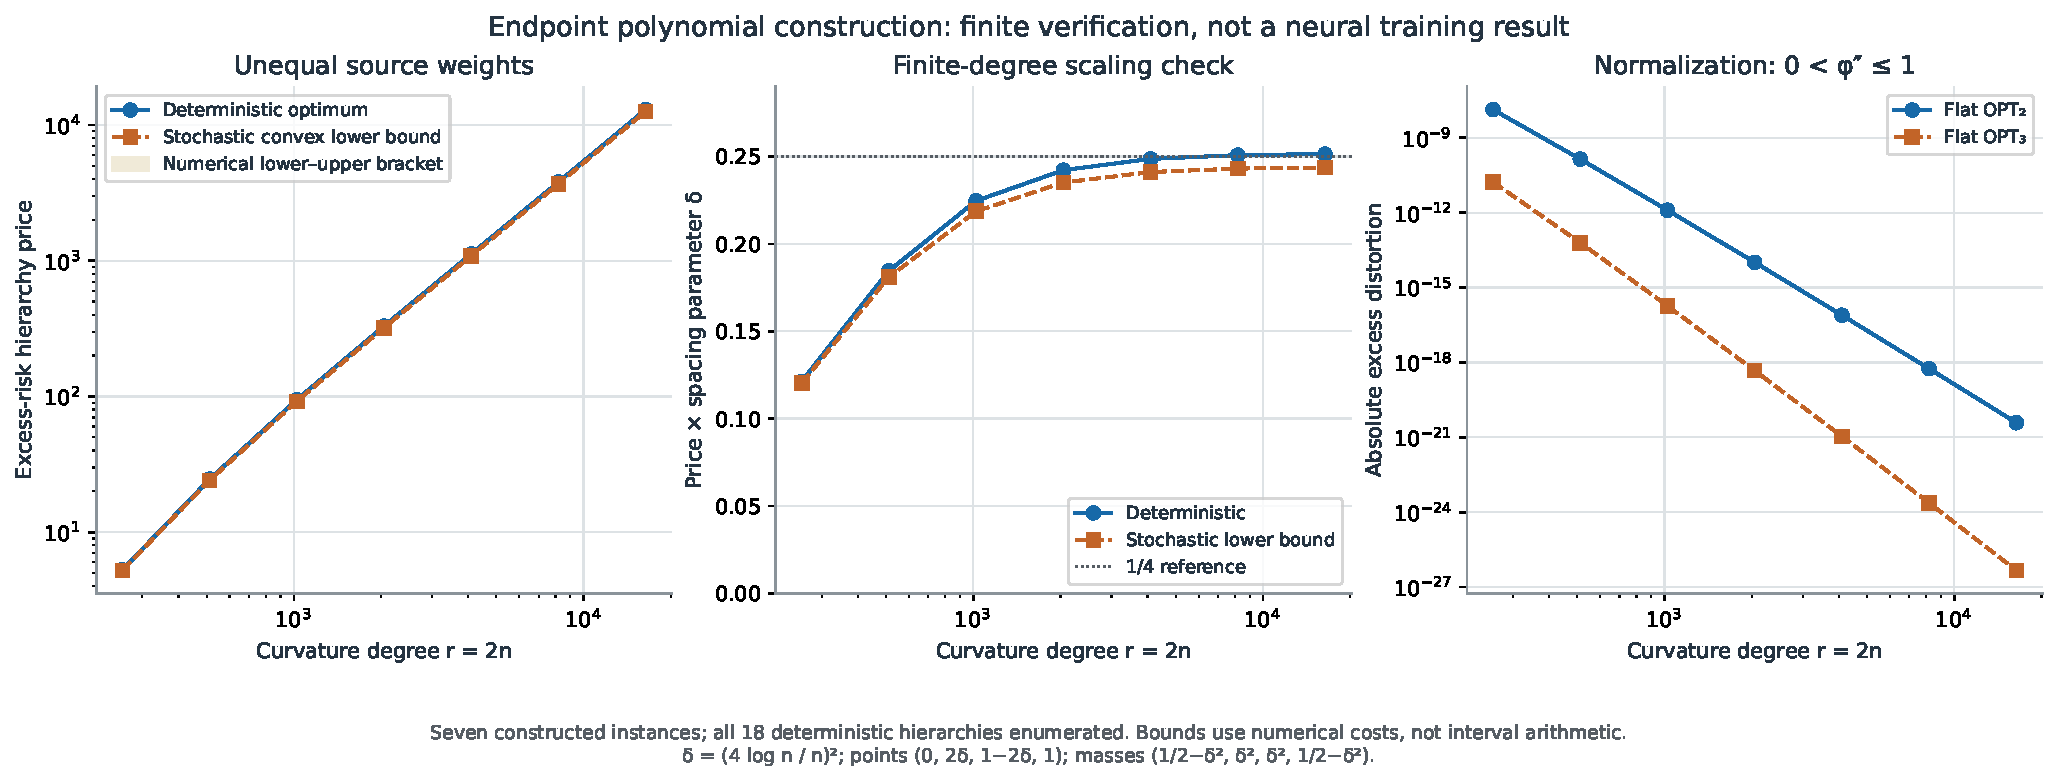
\includegraphics[width=\textwidth]{figures/endpoint_construction.pdf}
\caption{Endpoint family: numerical prices, prices multiplied by
$d_n$ (denoted $\delta$ in the plot), and normalized flat denominators.
The $1/4$ line is a visual reference, not a theorem. All eighteen
deterministic choices are enumerated; floating-point costs are independently
crosschecked as described in the text.}
\label{fig:endpoint}
\end{figure}

\subsection{Equal-mass controls and failed over-localization}
The original interior sequence uses $\varepsilon_n=16\log n/n$ and requires
$\varepsilon_n\le1/16$. The first integer $n\ge2$ meeting that condition is
$1938$, corresponding to curvature degree $7752$. Table~\ref{tab:equalnumerics}
reports the three sampled admissible members of that sequence.

\begin{table}[ht]
\centering\small
\begin{tabular}{@{}rrrrr@{}}
\toprule
$r=4n$ & $\varepsilon_n$ & Deterministic & Stochastic bracket & $n/(32\log n)$ \\
\midrule
8192 & 0.0595673 & 7.26645 & $[4.58790,5.53026]$ & 8.39386 \\
16384 & 0.0324913 & 14.1023 & $[8.07689,9.02771]$ & 15.3887 \\
32768 & 0.0175994 & 27.0290 & $[14.5837,15.5383]$ & 28.4100 \\
\bottomrule
\end{tabular}
\caption{Original equal-mass interior sequence. The last column is its
proved deterministic leading term, not a finite-degree equality. Stochastic
brackets use the convex lower construction and an explicit feasible channel.}
\label{tab:equalnumerics}
\end{table}

The full twenty-eight-case width scan includes distinct control families.
At fixed $\varepsilon=1/16$, price is $1$ at $r=64$, $1.00544$ at $r=128$,
and approaches $6.88889$ at the larger sampled degrees. Increasing degree
with fixed width therefore does not reproduce the diverging sequence.
At $n=8192$, width $\varepsilon_n/4$ gives price $112.170$, whereas the
narrower width $\varepsilon_n/8$ gives only $2.12227$ despite a hinge-reference
prediction of $225.795$. Finite-degree leakage defeats the excessively
narrow construction. These controls are different generators, not
lower-degree members of the original sequence. A separate twenty-four-case
spacing/weight screen contains many compatible instances of price one;
small inner weights alone need not create a conflict for a fixed curvature.

\begin{figure}[ht]
\centering
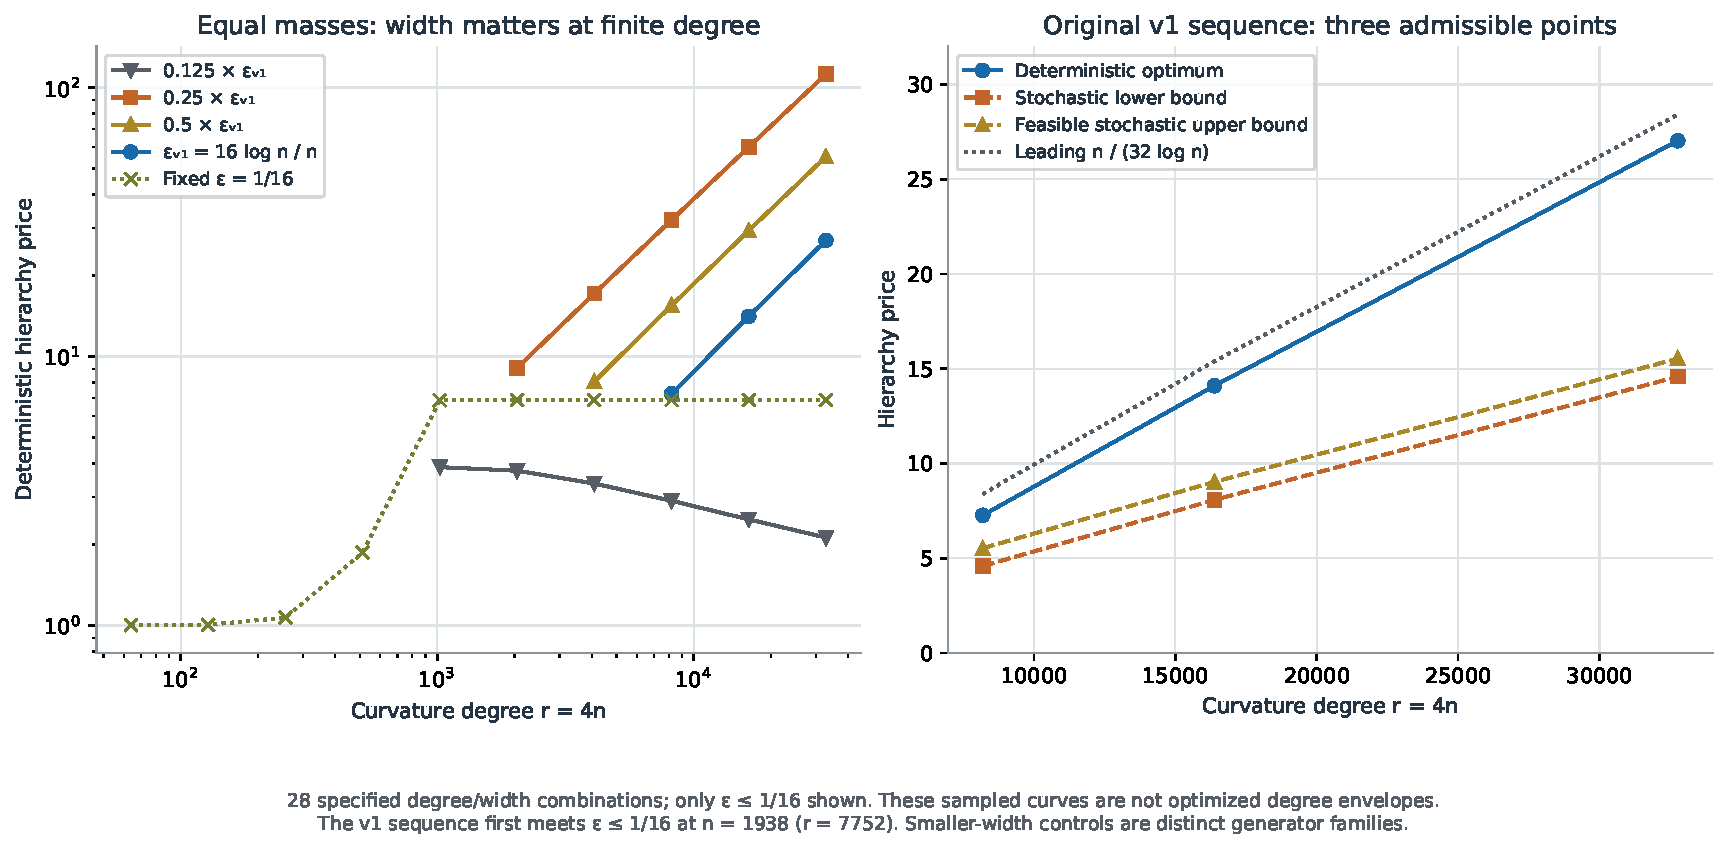
\includegraphics[width=\textwidth]{figures/equal_mass_degree_width.pdf}
\caption{Equal-mass finite-degree controls. The plotted curves are sampled
families, not optimized envelopes. The right panel uses only the three
admissible sampled members of the original interior sequence.}
\label{fig:equalcontrols}
\end{figure}

The uniform upper proof has intentionally loose constants:
$\log K=\log64+100\pi\log512\approx1963.986364$ in
\eqref{eq:logimplicit}. These experiments cannot certify its practical
threshold or either envelope's optimal leading constant. They also do not
numerically test the arbitrary-source all-capacity theorem.

\subsection{Reproduction and the representation-learning interface}
The companion script \path{research/experiments/code/reproduce.sh} reruns
the computations using an already available Python environment; no
installation or training is performed. The actual environment was Python
3.12.14 with NumPy 2.3.5, SciPy 1.18.1, mpmath, and Matplotlib 3.11.2.
Configuration files and logs preserve seeds, commands, environment versions,
and source hashes. Calculations used one main process and one-thread
BLAS/OpenMP caps; the successful recorded numerical phases took about
$31.5$ seconds in total, excluding startup and figure rendering. This is an
execution record rather than a performance benchmark.

The connection to representation learning requires a specified finite
state representation, source masses, Bernoulli posteriors, decoder, and
coarsening relation. If neuron growth is modeled as splitting cells of an
existing partition, the oracle Jensen costs quantify the price of retaining
that partition across capacities. Counting neurons does not itself supply
this finite-output model, and a learned predictor need not achieve the
oracle costs. Neither these calculations nor the hierarchy theorems imply
that a neuron-splitting rule improves training or population risk. A separate
learning experiment would need an explicit optimization and decoder model,
statistical error control, and a data-access and memory budget.
